\textbf{16/10/2026 (Clase 10)}
\section{Aplicaciones de la teoría de homotopía}

\subsection{Retractos y el teorema del punto fijo de Brouwer}

\begin{definicion}{Retracto [C10.1]}{def_retracto}
Sea $A \subseteq X$, con $X$ espacio topológico. Diremos que $A$ es un \textbf{retracto} de $X$ cuando existe una aplicación continua $r \colon X \to A$ tal que $r|_A = 1_A$, es decir, $r(a) = a$ para todo $a \in A$.
\end{definicion}

\begin{teorema}{No retracción en dimensión 2 [C10.2] \marcaT}{teo_no_retracto}
No existe ninguna aplicación continua $D^2 \to S^1$ cuya restricción a $S^1$ coincida con la identidad de $S^1$. Equivalentemente, $S^1$ no es un retracto de $D^2$.
\end{teorema}

\begin{proof}
Supongamos que existe $r \colon D^2 \to S^1$ continua con $r|_{S^1} = 1_{S^1}$. Sea $i \colon S^1 \to D^2$ la inclusión, de modo que $r \circ i = 1_{S^1}$. Fijado $x_0 \in S^1$, por funtorialidad
\[ r_{*,x_0} \circ i_{*,x_0} = (r \circ i)_{*,x_0} = (1_{S^1})_{*,x_0} = 1_{\pi_1(S^1,x_0)}. \]
Pero $i_{*,x_0} \colon \pi_1(S^1,x_0) \cong \mathbb{Z} \to \pi_1(D^2,x_0) = 1$, de modo que la identidad de $\mathbb{Z}$ factoriza a través del grupo trivial, lo cual es absurdo.
\begin{center}
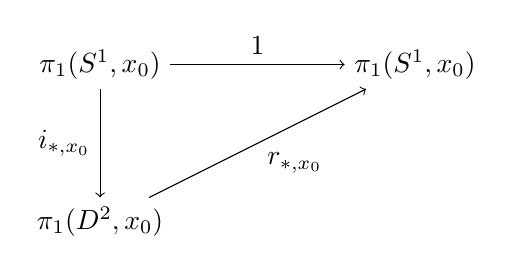
\begin{tikzpicture}
\node (A) at (0,2) {$\pi_1(S^1,x_0)$};
\node (B) at (4,2) {$\pi_1(S^1,x_0)$};
\node (C) at (0,0) {$\pi_1(D^2,x_0)$};
\draw[->] (A) -- (B) node[midway, above] {$1$};
\draw[->] (A) -- (C) node[midway, left] {$i_{*,x_0}$};
\draw[->] (C) -- (B) node[midway, below right] {$r_{*,x_0}$};
\end{tikzpicture}
\end{center}
\end{proof}

\begin{teorema}{Punto fijo de Brouwer [C10.3] \marcaT}{teo_brouwer}
Sea $f \colon D^2 \to D^2$ continua. Entonces existe $x_0 \in D^2$ tal que $f(x_0) = x_0$.
\end{teorema}

\begin{proof}
Supongamos que $f(x) \neq x$ para todo $x \in D^2$, es decir, $f(x) - x \neq 0$. Para cada $x \in D^2$ sea $r_x$ la semirrecta que parte de $f(x)$ con vector director $x - f(x)$, y sea $\varphi(x)$ el punto de intersección de $r_x$ con $S^1$ (el punto de salida del disco).

Escribimos $r_x = \{ f(x) + \lambda (x - f(x)) : \lambda \in [0,+\infty[ \}$. Un punto de $r_x$ tiene módulo $1$ cuando $\lambda$ vale
\[ \lambda = \frac{-f(x) \cdot (x - f(x)) + \sqrt{\big(f(x) \cdot (x - f(x))\big)^2 + \|x - f(x)\|^2 \big(1 - \|f(x)\|^2\big)}}{\|x - f(x)\|^2}. \]
Esta expresión analítica muestra que $\lambda$, y por tanto $\varphi$, es continua. Además, si $x \in S^1$ entonces $\varphi(x) = x$ (para $x \in S^1$ se tiene $f(x)\cdot(x-f(x)) \le 0$, y el valor $\lambda = 1$ es la raíz mayor). Luego $\varphi \colon D^2 \to S^1$ es continua y $\varphi|_{S^1} = 1_{S^1}$, lo que contradice el teorema anterior.
\end{proof}

\subsection{Teorema fundamental del álgebra}

\begin{teorema}{Teorema fundamental del álgebra [C10.5] \marcaT}{teo_fund_algebra}
Todo polinomio no constante de $\mathbb{C}[z]$ tiene al menos una raíz en $\mathbb{C}$.
\end{teorema}

\begin{proposicion}{Lema (cota de las raíces) [C10.4] \marcaL}{lema_cota_raices}
Sea $P(z) \in \mathbb{C}[z]$ mónico y no constante, de grado $k \geq 1$:
\[ P(z) = z^k + a_1 z^{k-1} + \dots + a_{k-1} z + a_k. \]
Si $z_0 \in \mathbb{C}$ cumple $P(z_0) = 0$, entonces $|z_0| < 1 + |a_1| + |a_2| + \dots + |a_k|$.
\end{proposicion}

\begin{proof}
Si $a_1 = \dots = a_k = 0$, la desigualdad es trivial ($0 < 1$). Supongamos que no todos los coeficientes son nulos y distingamos casos. Si $|z_0| \leq 1$, entonces $|z_0| \leq 1 < 1 + |a_1| + \dots + |a_k|$. Si $|z_0| > 1$:
\[ |z_0^k| = |-a_1 z_0^{k-1} - a_2 z_0^{k-2} - \dots - a_k| \leq |a_1||z_0|^{k-1} + \dots + |a_k|. \]
Dividiendo por $|z_0|^{k-1}$:
\[ |z_0| \leq |a_1| + |a_2|\frac{1}{|z_0|} + \dots + |a_k| \frac{1}{|z_0|^{k-1}} < |a_1| + |a_2| + \dots + |a_k| < 1 + |a_1| + \dots + |a_k|. \]
\end{proof}

\begin{proof}[Demostración del teorema fundamental del álgebra]
Sin pérdida de generalidad podemos suponer que $P(z)$ es mónico. Escribimos
\[ P(z) = z^k + a_1 z^{k-1} + \dots + a_{k-1} z + a_k, \qquad a_1,\dots,a_k \in \mathbb{C},\ k \geq 1. \]
Para $t \in [0,1]$ sea $P_t(z) = z^k + t a_1 z^{k-1} + t a_2 z^{k-2} + \dots + t a_{k-1} z + t a_k$, y sea $r := 1 + |a_1| + |a_2| + \dots + |a_k|$. Por el lema anterior, $P_t^{-1}(0) \subseteq B(0,r)$ para todo $t$; en particular, $P_t$ no se anula en la circunferencia $S^1_r = \{x \in \mathbb{R}^2 : \|x\| = r\}$.

Consideramos el lazo $\alpha \colon I \to S^1_r$, $\alpha(s) = r e^{2\pi i s}$, basado en $(r,0)$. Definimos
\[ H \colon I \times I \to S^1, \qquad H(s,t) = \frac{P_t(\alpha(s))}{P_t(r)} \cdot \left| \frac{P_t(r)}{P_t(\alpha(s))} \right|. \]
\begin{enumerate}
    \item $H$ es continua.
    \item $H_0(s) = \dfrac{\alpha(s)^k}{r^k} \cdot \dfrac{r^k}{|\alpha(s)|^k} = \left( \dfrac{\alpha(s)}{r} \right)^k = e^{2\pi i s k} =: w_k(s)$, con $w_k \colon I \to S^1$, $s \mapsto e^{2\pi i s k}$.
    \item $H_1(s) = \dfrac{P(\alpha(s))}{P(r)} \cdot \dfrac{|P(r)|}{|P(\alpha(s))|} =: \sigma(s)$.
    \item $H(0,t) = \dfrac{P_t(r)}{P_t(r)} \cdot \dfrac{|P_t(r)|}{|P_t(r)|} = 1$, no depende de $t$ (pues $\alpha(0) = r$).
    \item $H(1,t) = 1$, no depende de $t$ (pues $\alpha(1) = r$).
\end{enumerate}
Por (1)--(5), $H \colon w_k \simeq_{\{0,1\}} \sigma$, luego $\deg(\sigma) = \deg(w_k) = k$.

Supongamos ahora que $P(z)$ no tiene raíces en $\mathbb{C}$. Consideramos
\[ F \colon I \times I \to S^1, \qquad F(s,t) = \frac{P(t\,\alpha(s))}{P(t\,r)} \cdot \left| \frac{P(t\,r)}{P(t\,\alpha(s))} \right|, \]
que está bien definida por no haber raíces (en particular $a_k = P(0) \neq 0$).
\begin{enumerate}
    \item $F$ es continua.
    \item $F(s,0) = \dfrac{P(0)}{P(0)} \cdot \dfrac{|P(0)|}{|P(0)|} = 1$.
    \item $F(s,1) = \dfrac{P(\alpha(s))}{P(r)} \cdot \dfrac{|P(r)|}{|P(\alpha(s))|} = \sigma(s)$.
    \item $F(0,t) = 1$, no depende de $t$.
    \item $F(1,t) = 1$, no depende de $t$.
\end{enumerate}
Luego $F \colon c_1 \simeq_{\{0,1\}} \sigma$ y, por tanto, $\deg(c_1) = \deg(\sigma)$. Pero $\deg(c_1) = 0$, así que $0 = k \geq 1$, lo cual es absurdo. Concluimos que $P$ tiene alguna raíz en $\mathbb{C}$.
\end{proof}

\subsection{El grado no depende de la elevación}

En la \cref{def:def_grado} el grado solo se define para lazos basados en $(1,0)$, usando la elevación que empieza en $0$. Lo extendemos a cualquier punto base.

\begin{proposicion}{Lema (dos elevaciones) [C10.6] \marcaP}{lema_dos_elevaciones}
Sea $\omega \colon I \to S^1$ continua y sean $\tilde{\omega}_1, \tilde{\omega}_2$ dos elevaciones de $\omega$. Entonces existe $k \in \mathbb{Z}$ tal que $\tilde{\omega}_1 = \tilde{\omega}_2 + k$. En particular, $\tilde{\omega}_1(1) - \tilde{\omega}_1(0) = \tilde{\omega}_2(1) - \tilde{\omega}_2(0)$.
\end{proposicion}

\begin{proof}
Como $\tilde{\omega}_1,\tilde{\omega}_2$ son elevaciones de $\omega$, para cada $t \in I$
\[ p(\tilde{\omega}_1(t)) = \omega(t) = p(\tilde{\omega}_2(t)), \quad\text{es decir,}\quad e^{2\pi i \tilde{\omega}_1(t)} = e^{2\pi i \tilde{\omega}_2(t)}. \]
Luego existe $k(t) \in \mathbb{Z}$ con $2\pi i\,\tilde{\omega}_1(t) = 2\pi i\,\tilde{\omega}_2(t) + 2\pi i\,k(t)$, esto es, $k(t) = \tilde{\omega}_1(t) - \tilde{\omega}_2(t) \in \mathbb{Z}$. Automáticamente hemos definido una aplicación continua $k \colon I \to \mathbb{Z}$, luego $k$ es constante (por conexión). Así existe $k \in \mathbb{Z}$ con $\tilde{\omega}_1(t) = \tilde{\omega}_2(t) + k$ para todo $t \in I$, y
\[ \tilde{\omega}_1(1) - \tilde{\omega}_1(0) = \tilde{\omega}_2(1) + k - \tilde{\omega}_2(0) - k = \tilde{\omega}_2(1) - \tilde{\omega}_2(0). \]
\end{proof}

\begin{definicion}{Grado en un punto base cualquiera [C10.7]}{def_grado_x0}
Sean $x_0 \in S^1$ y $\alpha \in C_{x_0}(S^1)$. Definimos $\deg_{x_0}(\alpha) := \tilde{\alpha}(1) - \tilde{\alpha}(0)$, siendo $\tilde{\alpha}$ \emph{cualquier} elevación de $\alpha$ (está bien definido por el lema anterior).
\end{definicion}

\begin{teorema}{Cambio de punto base y grado [C10.9]}{teo_cambio_base_grado}
Sea $x_0 \in S^1$ y sea $\omega \colon I \to S^1$ una aplicación continua con $\omega(0) = x_0$ y $\omega(1) = (1,0)$. El diagrama
\begin{center}
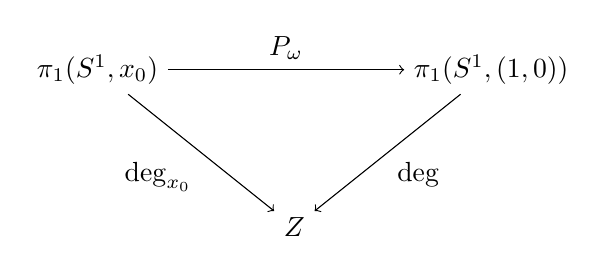
\begin{tikzpicture}
\node (A) at (0,2) {$\pi_1(S^1,x_0)$};
\node (B) at (5,2) {$\pi_1(S^1,(1,0))$};
\node (C) at (2.5,0) {$\mathbb{Z}$};
\draw[->] (A) -- (B) node[midway, above] {$P_\omega$};
\draw[->] (A) -- (C) node[midway, below left] {$\deg_{x_0}$};
\draw[->] (B) -- (C) node[midway, below right] {$\deg$};
\end{tikzpicture}
\end{center}
conmuta, es decir, $P_\omega([\alpha]) = [\omega^{-1} * \alpha * \omega] \in \pi_1(S^1,(1,0))$ y $\deg_{x_0}(\alpha) = \deg(\omega^{-1} * \alpha * \omega)$.
\end{teorema}

\textbf{23/10/2026 (Clase 12)} \quad \textit{(el ejercicio propuesto el 16/10 y planteado el 21/10)}

\begin{proof}
Basta probar que $\deg(\omega^{-1} * \alpha * \omega) = \deg_{x_0}(\alpha)$ para todo $\alpha \in C_{x_0}(S^1)$, pues $P_\omega([\alpha]) = [\omega^{-1} * \alpha * \omega]$. Consideramos tres elevaciones:
\begin{itemize}
    \item $\widetilde{\omega^{-1}} \colon I \to \mathbb{R}$, la elevación de $\omega^{-1}$ con $\widetilde{\omega^{-1}}(0) = 0$ (existe porque $\omega^{-1}(0) = (1,0)$, por la elevación de arcos);
    \item $\tilde{\alpha}$, la elevación de $\alpha$ con $\tilde{\alpha}(0) = \widetilde{\omega^{-1}}(1)$ (es posible porque $\widetilde{\omega^{-1}}(1) \in p^{-1}(\omega^{-1}(1)) = p^{-1}(x_0)$);
    \item $\tilde{\omega}$, la elevación de $\omega$ con $\tilde{\omega}(0) = \tilde{\alpha}(1)$.
\end{itemize}
Con estas condiciones, $\widetilde{\omega^{-1}} * \tilde{\alpha} * \tilde{\omega}$ está definida y es continua, y es una elevación de $\omega^{-1} * \alpha * \omega$, pues
\[ p \circ (\widetilde{\omega^{-1}} * \tilde{\alpha} * \tilde{\omega}) = (p \circ \widetilde{\omega^{-1}}) * (p \circ \tilde{\alpha}) * (p \circ \tilde{\omega}) = \omega^{-1} * \alpha * \omega. \]
Como empieza en $0$, el grado se obtiene evaluando en $1$:
\[ \deg(\omega^{-1} * \alpha * \omega) = (\widetilde{\omega^{-1}} * \tilde{\alpha} * \tilde{\omega})(1) - (\widetilde{\omega^{-1}} * \tilde{\alpha} * \tilde{\omega})(0) = \tilde{\omega}(1) - \widetilde{\omega^{-1}}(0) = \tilde{\omega}(1). \]
Falta ver que $\tilde{\omega}(1) = \tilde{\alpha}(1) - \tilde{\alpha}(0)$, que es lo que hay que comprobar para que este grado coincida con $\deg_{x_0}(\alpha)$.

La aplicación $(\widetilde{\omega^{-1}})^{-1}$, dada por $t \mapsto \widetilde{\omega^{-1}}(1-t)$, es otra elevación de $\omega$:
\[ \big(p \circ (\widetilde{\omega^{-1}})^{-1}\big)(t) = p\big(\widetilde{\omega^{-1}}(1-t)\big) = \omega^{-1}(1-t) = \omega(t). \]
Por el \cref{prop:lema_dos_elevaciones}, $\tilde{\omega}$ y $(\widetilde{\omega^{-1}})^{-1}$ tienen el mismo incremento entre $0$ y $1$:
\[ \tilde{\omega}(1) - \tilde{\omega}(0) = (\widetilde{\omega^{-1}})^{-1}(1) - (\widetilde{\omega^{-1}})^{-1}(0) = \widetilde{\omega^{-1}}(0) - \widetilde{\omega^{-1}}(1) = -\tilde{\alpha}(0). \]
Como $\tilde{\omega}(0) = \tilde{\alpha}(1)$, queda $\tilde{\omega}(1) = \tilde{\alpha}(1) - \tilde{\alpha}(0) = \deg_{x_0}(\alpha)$.
\end{proof}

\begin{observacion}{$\deg_{x_0}$ solo depende de la clase}{obs_grado_clase}
Por el teorema anterior, $\deg_{x_0}(\alpha) = \deg(\omega^{-1} * \alpha * \omega)$ y la clase $[\omega^{-1} * \alpha * \omega] = P_\omega([\alpha])$ solo depende de $[\alpha]$. Por tanto, si $\alpha \simeq_{\{0,1\}} \beta$ en $C_{x_0}(S^1)$, entonces $\deg_{x_0}(\alpha) = \deg_{x_0}(\beta)$. Se usa en el corolario de la no existencia de aplicaciones impares.
\end{observacion}

\subsection{Funciones pares e impares: el teorema de paridad}

\begin{definicion}{Conjunto simétrico, función par e impar [C10.10]}{def_par_impar}
Sea $A \subseteq \mathbb{R}^n$. Diremos que $A$ es \textbf{simétrico} cuando $x \in A \implies -x \in A$. Sea $f \colon A \to \mathbb{R}^m$ con $A$ simétrico. Diremos que $f$ es \textbf{par} cuando $f(x) = f(-x)$ para todo $x \in A$, e \textbf{impar} cuando $f(x) = -f(-x)$ para todo $x \in A$.
\end{definicion}

\begin{teorema}{De paridad de Borsuk--Hirsch [C10.11] \marcaT}{teo_paridad}
Sea $\sigma \colon I \to S^1$, $\sigma(s) = e^{2\pi i s}$ para todo $s \in I$, y sea $f \colon S^1 \to S^1$ continua. Entonces:
\begin{enumerate}
    \item[a)] Si $f$ es par, entonces $\deg(f \circ \sigma)$ es par.
    \item[b)] Si $f$ es impar, entonces $\deg(f \circ \sigma)$ es impar.
\end{enumerate}
\end{teorema}

\textbf{21/10/2026 (Clase 11)}

\begin{proof}
Sea $z := f \circ \sigma$. Como $z(0) = f(\sigma(0)) = f(1) = f(\sigma(1)) = z(1)$, $z$ es un lazo basado en $f(1)$ y $\deg(z)$ significa $\deg_{f(1)}(z)$ (\cref{def:def_grado_x0}). Sea $\tilde{z} \colon I \to \mathbb{R}$ cualquier elevación de $z$, de modo que $\deg(z) = \tilde{z}(1) - \tilde{z}(0)$. Para $t \in [0,\frac12]$ se tiene $\sigma(\frac12 + t) = e^{\pi i} e^{2\pi i t} = -\sigma(t)$, luego
\[ z\left(\tfrac12 + t\right) = f\left(-\sigma(t)\right). \]

\textbf{a)} Supongamos que $f$ es par. Entonces $z(\frac12 + t) = f(-\sigma(t)) = f(\sigma(t)) = z(t)$. Definimos $h \colon [0,\frac12] \to \mathbb{R}$, $h(t) = \tilde{z}(\frac12 + t) - \tilde{z}(t)$. Entonces
\[ (p \circ h)(t) = e^{2\pi i \tilde{z}(\frac12 + t)} \, e^{-2\pi i \tilde{z}(t)} = \frac{z(\frac12 + t)}{z(t)} = 1, \]
luego $h(t) \in p^{-1}(1) = \mathbb{Z}$ para todo $t$. Como $h$ es continua y $[0,\frac12]$ es conexo, $h$ es constante: existe $k \in \mathbb{Z}$ con $h(t) = k$ para todo $t$. Por tanto
\[ \deg(z) = \tilde{z}(1) - \tilde{z}(0) = \big(\tilde{z}(\tfrac12 + \tfrac12) - \tilde{z}(\tfrac12)\big) + \big(\tilde{z}(\tfrac12) - \tilde{z}(0)\big) = h(\tfrac12) + h(0) = 2k, \]
que es par.

\textbf{b)} Supongamos que $f$ es impar. Entonces $z(\frac12 + t) = f(-\sigma(t)) = -f(\sigma(t)) = -z(t)$. Definimos $g \colon [0,\frac12] \to \mathbb{R}$, $g(t) = \tilde{z}(\frac12 + t) - \tilde{z}(t) - \frac12$. Entonces
\[ (p \circ g)(t) = \frac{z(\frac12 + t)}{z(t)} \cdot e^{-\pi i} = (-1)(-1) = 1, \]
luego $g$ toma valores en $\mathbb{Z}$ y, por conexión, es constante igual a un $k \in \mathbb{Z}$. Así
\[ \deg(z) = \tilde{z}(1) - \tilde{z}(0) = \big(\tilde{z}(1) - \tilde{z}(\tfrac12) - \tfrac12\big) + \big(\tilde{z}(\tfrac12) - \tilde{z}(0) - \tfrac12\big) + 1 = g(\tfrac12) + g(0) + 1 = 2k + 1, \]
que es impar.
\end{proof}

\subsection{Consecuencias del teorema de paridad}

\begin{proposicion}{No existen aplicaciones impares $S^2 \to S^1$ [C11] \marcaC}{cor_no_impar}
No existe ninguna aplicación continua impar $S^2 \to S^1$.
\end{proposicion}

\begin{proof}
Supongamos que existe $g \colon S^2 \to S^1$ continua con $g(-x) = -g(x)$ para todo $x \in S^2$. Sea $\sigma \colon I \to S^1$ el lazo estándar y sea $j \colon S^1 \to S^2$, $j(x,y) = (x,y,0)$. Definimos $f := g \circ j \colon S^1 \to S^1$. Es impar:
\[ f(-p) = g(j(-p)) = g(-p,0) = g(-(p,0)) = -g(p,0) = -f(p). \]
Por el \cref{thm:teo_paridad}, $\deg(f \circ \sigma)$ es impar.

Por otro lado, $j \circ \sigma$ es un lazo en $S^2$ basado en $(1,0,0)$, pues $j(\sigma(0)) = j(\sigma(1)) = (1,0,0)$. Como $S^2$ es simplemente conexo (\cref{prop:corolario_sn}), $\pi_1(S^2,(1,0,0)) = 1$, así que existe una homotopía $H \colon I \times I \to S^2$ con $H \colon j \circ \sigma \simeq_{\{0,1\}} c_{(1,0,0)}$. Componiendo con $g$, la aplicación $g \circ H$ es una homotopía relativa entre
\[ g \circ j \circ \sigma = f \circ \sigma \qquad\text{y}\qquad g \circ c_{(1,0,0)} = c_{g(1,0,0)}. \]
Por la \cref{obs:obs_grado_clase}, $\deg(f \circ \sigma) = \deg(c_{g(1,0,0)}) = 0$, que es par. Contradicción.
\end{proof}

\begin{proposicion}{Ceros de aplicaciones impares [C11] \marcaC}{cor_cero_impar}
Sea $f \colon S^2 \to \mathbb{R}^2$ continua e impar. Entonces existe $x_0 \in S^2$ con $f(x_0) = 0$.
\end{proposicion}

\begin{proof}
Supongamos que $f(x) \neq 0$ para todo $x \in S^2$. Entonces $g \colon S^2 \to S^1$, $g(x) = \frac{f(x)}{\|f(x)\|}$, es continua y
\[ g(-x) = \frac{f(-x)}{\|f(-x)\|} = \frac{-f(x)}{\|f(x)\|} = -g(x), \]
es decir, $g$ es impar, lo que contradice la \cref{prop:cor_no_impar}.
\end{proof}

\begin{teorema}{de Borsuk [C11] \marcaC}{teo_borsuk}
Sea $f \colon S^2 \to \mathbb{R}^2$ continua. Entonces existe $x \in S^2$ tal que $f(x) = f(-x)$.
\end{teorema}

\begin{proof}
Supongamos que $f(x) \neq f(-x)$ para todo $x \in S^2$. Entonces $g \colon S^2 \to S^1$, $g(x) = \frac{f(x) - f(-x)}{\|f(x) - f(-x)\|}$, es continua y
\[ g(-x) = \frac{f(-x) - f(x)}{\|f(-x) - f(x)\|} = -g(x), \]
luego $g$ es impar, lo que contradice la \cref{prop:cor_no_impar}.
\end{proof}

\begin{proposicion}{No hay inyectivas $S^2 \to \mathbb{R}^2$ [C11] \marcaC}{cor_no_inyectiva}
No existe ninguna aplicación continua e inyectiva $f \colon S^2 \to \mathbb{R}^2$. En particular, no existe ninguna aplicación continua e inyectiva $S^2 \to S^1$.
\end{proposicion}

\begin{proof}
Por el teorema de Borsuk existe $x \in S^2$ con $f(x) = f(-x)$, y $x \neq -x$, luego $f$ no es inyectiva. El caso $S^2 \to S^1$ se obtiene viendo $S^1 \subseteq \mathbb{R}^2$.
\end{proof}

\begin{observacion}{Aplicación a la Tierra [C11]}{obs_tierra}
Como consecuencia del teorema de Borsuk, si la Tierra fuera una esfera perfecta, en todo momento existirían dos puntos antipodales con exactamente la misma temperatura y la misma presión (basta tomar $f$ = (temperatura, presión), continua de $S^2$ en $\mathbb{R}^2$).
\end{observacion}

\begin{proposicion}{Continuidad de la distancia a un conjunto [C11] \marcaL}{lema_dist_continua}
Sea $\emptyset \neq C \subseteq \mathbb{R}^n$ y sea $f \colon \mathbb{R}^n \to \mathbb{R}_{\geq 0}$, $f(x) = d(x,C) = \inf_{y \in C} \|x - y\|$. Entonces $f$ es continua (de hecho, uniformemente continua).
\end{proposicion}

\begin{proof}
Sean $x_0, x \in \mathbb{R}^n$. Para todo $y \in C$, $\|x_0 - y\| \leq \|x_0 - x\| + \|x - y\|$. Tomando ínfimos en $y \in C$, $d(x_0,C) \leq \|x_0 - x\| + d(x,C)$. Análogamente, $d(x,C) \leq \|x - x_0\| + d(x_0,C)$. Luego $|f(x) - f(x_0)| \leq \|x - x_0\|$, y dado $\varepsilon > 0$ basta tomar $\delta = \varepsilon$.
\end{proof}

\begin{teorema}{de Lyusternik--Schnirelmann [C11] \marcaC}{teo_lyusternik}
Si $A_1, A_2, A_3$ son cerrados de $S^2$ con $S^2 = A_1 \cup A_2 \cup A_3$, entonces existen $i \in \{1,2,3\}$ y $p \in S^2$ tales que $\{p,-p\} \subseteq A_i$ (alguno de los tres cerrados contiene dos puntos antipodales).
\end{teorema}

\begin{proof}
\begin{enumerate}
    \item Si $C$ es cerrado en $S^2$, entonces es cerrado en $\mathbb{R}^3$, y para $x \in \mathbb{R}^3$ se tiene $x \in C \iff d(x,C) = 0$, donde $d(x,C) = \inf\{\|x - y\| : y \in C\}$.
    \item Consideramos $g \colon S^2 \to \mathbb{R}^2$, $g(x) = (d(x,A_1),\, d(x,A_2))$, continua por la \cref{prop:lema_dist_continua}.
    \item Por el teorema de Borsuk existe $x \in S^2$ con $g(x) = g(-x)$, es decir, $d(x,A_1) = d(-x,A_1)$ y $d(x,A_2) = d(-x,A_2)$.
    \item Si $d(x,A_1) = 0$, entonces $d(-x,A_1) = 0$ y $x, -x \in A_1$. Análogamente, si $d(x,A_2) = 0$, entonces $x, -x \in A_2$.
    \item Si $d(x,A_1) \neq 0$ y $d(x,A_2) \neq 0$, entonces $x \notin A_1 \cup A_2$ y, por la igualdad del paso 3, $-x \notin A_1 \cup A_2$. Como $S^2 = A_1 \cup A_2 \cup A_3$, resulta $x, -x \in A_3$.
\end{enumerate}
\end{proof}

\subsection{Grupos de homotopía y el conjunto $\pi_0$}

\textbf{23/10/2026 (Clase 12)}

El grupo fundamental se definió como $\pi_1(X,x_0) = C(X,x_0)/\simeq_{\{0,1\}}$, usando arcos $\alpha \colon I \to X$ con $I = [0,1]$. Cambiando $I$ por otros espacios se obtiene una familia de \textbf{grupos de homotopía} $\pi_*(X) = \{\pi_n(X,x_0)\}_{n \geq 0}$ (y se plantea calcular $\pi_*(S^n)$). Veamos la definición de $\pi_0(X)$.

Una \textbf{arco-componente} de $X$ es un subespacio arco-conexo maximal de $X$, es decir, un subespacio arco-conexo $C \subseteq X$ tal que si $D$ es arco-conexo y $C \subseteq D \subseteq X$, entonces $C = D$. Todo subespacio arco-conexo está contenido en una única arco-componente (si estuviera en dos, $A$ y $B$, la maximalidad da $A = B$).

\begin{definicion}{El conjunto $\pi_0(X)$ [C12]}{def_pi0}
Sea $C^{(0)}(X) = \{f \colon \{0\} \to X \text{ continua}\}$, que está en biyección con $X$ (se identifica $f$ con $f(0)$). Se define $\pi_0(X) := C^{(0)}(X)/\!\simeq$, donde $\simeq$ es la homotopía entre aplicaciones.
\end{definicion}

Dos aplicaciones $f, g \colon \{0\} \to X$ son homotópicas si y solo si $f(0)$ y $g(0)$ están conectados por un arco:
\begin{itemize}
    \item[$\Rightarrow)$] Si $F \colon \{0\} \times I \to X$ cumple $F_0 = f$ y $F_1 = g$, el arco $\alpha(t) = F(0,t)$ cumple $\alpha(0) = f(0)$ y $\alpha(1) = g(0)$.
    \item[$\Leftarrow)$] Si $\alpha \colon I \to X$ es un arco con $\alpha(0) = f(0)$ y $\alpha(1) = g(0)$, entonces $F(0,t) = \alpha(t)$ es una homotopía entre $f$ y $g$.
\end{itemize}
Por tanto, $\pi_0(X)$ \textbf{es el conjunto de las arco-componentes de $X$}.

\begin{proposicion}{$\#\pi_0$ es invariante homotópico [C12]}{prop_pi0_invariante}
Si $X \simeq Y$, entonces $\#\pi_0(X) = \#\pi_0(Y)$. (Referencia: Kosniowski, \emph{Topología algebraica}, Ed. Reverté.)
\end{proposicion}

\begin{proof}
Sean $f \colon X \to Y$ y $g \colon Y \to X$ continuas con $g \circ f \simeq 1_X$ y $f \circ g \simeq 1_Y$. Dada una aplicación continua $f \colon X \to Y$, definimos
\[ \pi_0(f) \colon \pi_0(X) \to \pi_0(Y), \qquad C \mapsto D_C, \]
donde $D_C$ es la única arco-componente de $Y$ con $f(C) \subseteq D_C$ (existe porque $f(C)$ es arco-conexo, por ser imagen continua de un arco-conexo, y está contenido en una única arco-componente). Basta probar, para $X \xrightarrow{f} Y \xrightarrow{g} Z$ aplicaciones cualesquiera:
\begin{enumerate}
    \item[\textcircled{1}] $\pi_0(g \circ f) = \pi_0(g) \circ \pi_0(f)$.
    \item[\textcircled{2}] $\pi_0(1_X) = 1_{\pi_0(X)}$.
    \item[\textcircled{3}] $f \simeq g \implies \pi_0(f) = \pi_0(g)$.
\end{enumerate}

\textcircled{1} Sea $C$ una arco-componente de $X$. Sea $D_C = \pi_0(f)(C)$, de modo que $f(C) \subseteq D_C$, y sea $E = \pi_0(g)(D_C)$, de modo que $g(D_C) \subseteq E$. Entonces $(g \circ f)(C) \subseteq g(D_C) \subseteq E$, y como $E$ es una arco-componente, es la única que contiene a $(g \circ f)(C)$, es decir, $\pi_0(g \circ f)(C) = E = \pi_0(g)(\pi_0(f)(C))$.

\textcircled{2} Para $C \in \pi_0(X)$, se tiene $1_X(C) = C \subseteq C$, luego $\pi_0(1_X)(C) = C$.

\textcircled{3} Sea $F \colon X \times I \to Y$ con $F_0 = f$ y $F_1 = g$, y sea $C \in \pi_0(X)$. Como $C \times I$ es arco-conexo, $F(C \times I)$ es arco-conexo, y está contenido en una única arco-componente $D$ de $Y$. Como $f(C) = F(C \times \{0\}) \subseteq D$ y $g(C) = F(C \times \{1\}) \subseteq D$, se tiene $\pi_0(f)(C) = D = \pi_0(g)(C)$.

Con \textcircled{1}--\textcircled{3}: de $g \circ f \simeq 1_X$ se obtiene $\pi_0(g) \circ \pi_0(f) = \pi_0(g \circ f) = \pi_0(1_X) = 1_{\pi_0(X)}$, y de $f \circ g \simeq 1_Y$, $\pi_0(f) \circ \pi_0(g) = 1_{\pi_0(Y)}$. Luego $\pi_0(f)$ es biyectiva con inversa $\pi_0(g)$, y $\#\pi_0(X) = \#\pi_0(Y)$.
\end{proof}

\subsection{Ejercicios resueltos en clase}

\begin{center}
\textbf{21/10/2026 (Clase 11)}
\end{center}

\begin{ejercicio}{Tema 5, ej. 3, apartado 1 (Borsuk en el toro)}
¿Se cumple el teorema de Borsuk en el toro $\mathbb{T}^2 \subseteq \mathbb{R}^3$? Es decir, ¿es cierto que para toda $f \colon \mathbb{T}^2 \to \mathbb{R}^2$ continua existe $x \in \mathbb{T}^2$ con $f(x) = f(-x)$?

\textbf{Respuesta: no.} Sea $g \colon \mathbb{R}^3 \to \mathbb{R}^2$, $g(x,y,z) = (x,y)$ y $f = g|_{\mathbb{T}^2}$. Si existiera $p = (p_1,p_2,p_3) \in \mathbb{T}^2$ con $g(p) = g(-p)$, entonces $(p_1,p_2) = (-p_1,-p_2)$, es decir, $p_1 = p_2 = 0$. Pero el toro no tiene ningún punto cuyas dos primeras coordenadas sean $0$. Luego esa $f$ no cumple la conclusión.
\end{ejercicio}

\begin{ejercicio}{Tema 5, ej. 3, apartado 2 ($f \colon S^1 \to \mathbb{R}$)}
Sea $f \colon S^1 \to \mathbb{R}$ continua. Probar que existe $x_0 \in S^1$ con $f(x_0) = f(-x_0)$.

\textbf{Solución.} Supongamos que $f(x) \neq f(-x)$ para todo $x \in S^1$. Definimos la aplicación continua
\[ g \colon S^1 \to \mathbb{R}, \qquad g(x) = \frac{f(x) - f(-x)}{|f(x) - f(-x)|}, \]
cuya imagen está contenida en $\{-1,1\}$. Como $S^1$ es conexo y $g$ es continua, $g(S^1)$ es conexo y está contenido en $\{-1,1\}$, luego $g$ es constante: $g(x) = k \in \{-1,1\}$ para todo $x$. Pero
\[ g(-x) = \frac{f(-x) - f(x)}{|f(-x) - f(x)|} = -g(x), \]
es decir, $k = -k$, luego $k = 0$, lo cual es absurdo.
\end{ejercicio}

\begin{center}
\textbf{23/10/2026 (Clase 12)}
\end{center}

\begin{ejercicio}{Tema 5, ej. 6 ($\#\pi_0$ es invariante homotópico)}
Probar que el cardinal del conjunto de arco-componentes de un espacio es un invariante homotópico. Es la \cref{prop:prop_pi0_invariante}.
\end{ejercicio}

\begin{ejercicio}{Tema 5, ej. 7 (conexo no arco-conexo)}
Sea $X = \{(x,\sin\frac1x) : x \in\, ]0,1]\} \cup (\{0\} \times [-1,1])$, la adherencia $\overline{A}$ de la gráfica $A$. Es un ejemplo clásico de espacio conexo que no es arco-conexo.

$X$ tiene $2$ arco-componentes (la gráfica y el segmento $\{0\} \times [-1,1]$). Por tanto $\#\pi_0(X) = 2 \neq 1 = \#\pi_0(\{p\})$, donde $\{p\}$ es un punto. Si $X$ fuese contráctil, tendría el mismo tipo de homotopía que un punto y, por la \cref{prop:prop_pi0_invariante}, $\#\pi_0(X) = 1$. Luego $X$ \textbf{no es contráctil}. (Los hechos sobre las arco-componentes de $X$ se enunciaron en clase sin demostración.)
\end{ejercicio}

\begin{ejercicio}{ejercicios propuestos el 16/10 sobre el grado}
\begin{itemize}
    \item $\deg_{x_0}(\alpha) = \deg_{x_0}(\beta)$ si $\alpha \simeq_{\{0,1\}} \beta$: es la \cref{obs:obs_grado_clase}.
    \item $\deg_{(1,0)} \circ P_\omega = \deg_{x_0}$: demostrado en el \cref{thm:teo_cambio_base_grado} (completado el 23/10).
\end{itemize}
\end{ejercicio}
